\subsubsection{Fra 3D-model til billede}
\label{sec:fra_model_til_billede}
I dette afsnit er det vist, hvordan der kan udledes en model, der beskriver en billeddannelsen af objekter i rummet, også kaldt rendering. Dette er essentielt da billeddannelsen danner grundlag for, hvordan 3D-modellen for en lampe omdannes til et billede, der kan vises for kunderne på e-butikken. Til sidst i afsnittet udledes en model for, hvordan belysningen fra en lampe kan simuleres og visualiseres vha. raytracing. 

\paragraph{3D-model}
En 3D-model er en matematisk beskrivelse af et tre dimensionelt objekt. For at beskrive et 3D-objekt opdeler man ofte objektet i trekanter. Dette er illustreret på nedenstående figur.

\begin{figure}[H]
\label{fig:kanin}
    \centering
    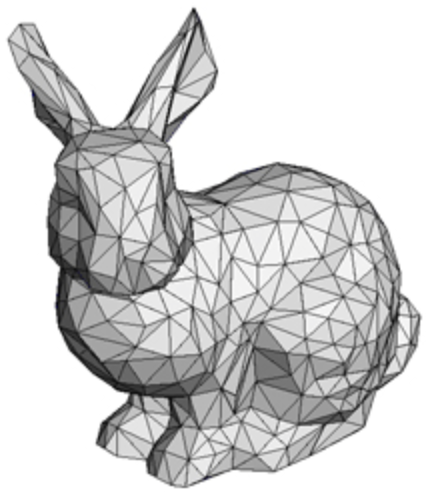
\includegraphics[width=5cm]{kanin}
    \caption{Eksempel hvor trekanter bruges til at repræsentere et objekt: http://www.cs.rpi.edu}
\end{figure}

For at rendere et billede af en 3D-model bestående af trekanter, er man nødt til at have en model for det kamera, som billedet renderes ud fra. Hvordan kameraet kan modelleres er beskrevet i næste afsnit.

\paragraph{Kamera}
[BESKRIV HVORDAN KAMERAET ER EN MODEL FOR HVORDAN DER LAVES ET BILLEDE AF ET KAMERA]
For at beskrive kameraet er det nødvendigt at fastlægge dets position og orientering i rummet[KILDE]. Hvordan dette kan modelleres er vist på figur [INDSÆT REF]

\begin{figure}[H]
  \centering
  \tdplotsetmaincoords{60}{130}
\begin{tikzpicture}[tdplot_main_coords]
\path[fill=gray!20, draw=gray!40] (-2,-4,-2) -- (-2,-4,2) -- (2,-4,2) -- (2,-4,-2) -- (-2,-4,-2);
\draw (0,0,0) -- (0,-4,0);
\draw[blue!50, thick, -{Stealth[width=2mm, length=2mm]}] (0,0,0) -- (0,-2,0);
\draw[blue!50, thick, -{Stealth[width=2mm, length=3mm]}] (0,-4,0) -- (-2,-4,0);
\draw[blue!50, thick, -{Stealth[width=2mm, length=2mm]}] (0,-4,0) -- (0,-4,2);
\draw plot [mark=*, mark size=2] coordinates{(0,0,0) }; 
\node [above right] at (0,0,0) {$C$};
\node [above right] at (0,-1,0) {$\vv{f}$};
\node [above] at (-1,-4,0) {$\vv{r}$};
\node [left] at (0,-4,1) {$\vv{u}$};
\end{tikzpicture}
  \caption{Viser hvordan kameraet kan beskrives ved tre vektorer $\protect\vv{r}$, $\protect\vv{u}$ og $\protect\vv{f}$, der repræsentere hhv. op, højre og frem retninger for kameraet.}
\label{fig:kamera_billede}
\end{figure}

[FIGUR TILFØJ VEKTORER DER BESKRIVER PUNKTET B, SOM LINEAR KOMBINATION.]

[SKRIV EN FORMEL DER VISER SAMMENHÆNGEN MELLEM ET PIXELKOORDINAT (X, Y) OG SÅ PUNKTET PÅ BILLEDPLANEN, UD FRA VEKTORERNE FOR KAMERAET.]

[SKRIV OVERGANG TIL NÆSTE AFSNIT]

\paragraph{Perspektiv projektion}
\label{sec:perspektiv_projektion}
For at udlede en model for billeddannelsen, tages der udgangspunkt i en perspektiv projektion. Perspektiv projektion er en måde at danne et billede af 3D-objekter ved at projektere objekterne hen på et plan mod et kameraes position\cite{fig:perspective_projection}. Princippet bag perspektiv projektion er vist på figur \ref{fig:perspektiv_projektion}.

\begin{figure}[H]
  \label{fig:perspektiv_projektion}
  \centering
  \tdplotsetmaincoords{60}{130}
\begin{tikzpicture}[tdplot_main_coords]
\path[fill=blue!50, draw=gray!20] (2,-8,2) -- (-2,-8,2) -- (0,-8,0) -- (2,-8,2);
\draw (0,0,0) -- (2,-8,2);
\path[fill=gray!20, draw=gray!40] (-2,-4,-2) -- (-2,-4,2) -- (2,-4,2) -- (2,-4,-2) -- (-2,-4,-2);
\path[fill=blue!50, draw=gray!20] (1,-4,1) -- (-1,-4,1) -- (0,-4,0) -- (1,-4,1);
\draw (0,0,0) -- (1,-4,1);

\draw plot [mark=*, mark size=2] coordinates{(2,-8,2) } ; 
\draw plot [mark=*, mark size=2] coordinates{(1,-4,1) }; 
\draw plot [mark=*, mark size=2] coordinates{(0,0,0) }; 
\node [above left] at (2,-8,2) {$P$};
\node [above left] at (1,-4,1) {$B$};
\node [above right] at (0,0,0) {$C$};
\end{tikzpicture}
  \caption{Viser princippet bag perspektiv projektion af et punkt på et billedplan.}
\end{figure}

[TEGN TO PUNKTER MERE PÅ FIGUREN OVENOVER OG TAG UDGANGSPUNKT I AFBILDNING AF EN TREKANT I STEDET FOR ET PUNKT.]

Som vist på figur \ref{fig:perspektiv_projektion} kan et punkt $P\in \mathbb{R}^3$ projekteres ned på billedplanen $\alpha$ ved at finde skæringspunktet $B$ mellem billedplanen $\alpha$ og en lysstråle $L$, som går fra punktet $P$ mod kameraets position $C$. Gør man nu dette for alle punkter på et objekt i rummet, og tegner skæringspunkterne på billedplanen, dannes et billede af objektet. For at omdanne 3D-objekter i rummet til et billede, er det nødvendigt at have en model for kameraet der danner billedet. 

Udfordringen er så at afgøre hvilken farve punkterne på billedplanen skal have, da dette afhænger af objektets egenskaber, samt hvilket udefrakommende lys der rammer objektet. 

For at løse denne udfordring, benytter vi i dette projekt raytracing, der som beskrevet under afsnit \ref{sec:computergrafik}, bygger på at simulere lysstrålers interaktion med forskellige objekter i rummet. Hvordan dette fungere er beskrevet i næste afsnit, hvor der er beskrevet en model for backwards raytracing.

\paragraph{Backwards raytracing}
I modsætning til en perspektiv projektion af et punkt på et plan, er backwards raytracing, hvor man i stedet for punktet i rummet, tager udgangspunkt i de lysstråler der danner billedet. Ved backwards raytracing følger man lysstrålerne baglæns og ser på, hvor stor en lysintensitet, den pågældende lysstråle har efter den har interageret med objekterne i rummet. Ud fra dette farves det tilhørende punkt på billedet, og på den måde kan man rendere et helt billede. På figur \ref{fig:raytracing_skitse} er det vist hvordan man kan konstruere en lysstråle ud fra et bestemt punkt på billedplanen, hvor lysstrålen er beskrevet ved en retningsvektor og et startpunkt.

\begin{figure}[H]
  \label{fig:raytracing_skitse}
  \centering
  \tdplotsetmaincoords{60}{130}
  \begin{tikzpicture}[tdplot_main_coords]
  \path[fill=blue!50, draw=gray!20] (2,-8,2) -- (-2,-8,2) -- (0,-8,0) -- (2,-8,2);
\draw (0,0,0) -- (0,-8,1);
\path[fill=gray!20, draw=gray!40] (-2,-4,-2) -- (-2,-4,2) -- (2,-4,2) -- (2,-4,-2) -- (-2,-4,-2);
\draw plot [mark=*, mark size=2] coordinates{(0,-4,0.5) }; 
\draw plot [mark=*, mark size=2] coordinates{(0,0,0) }; 
\node [above right] at (0,-4,0.5) {$B$};
\node [above right] at (0,0,0) {$C$};
\draw [blue!50, thick, -{Stealth[width=3mm, length=3mm]}] (0,0,0) -- (0,-4,0.5);
\node [above right] at (0,-2,0.25) {$\vv{r}$};
\end{tikzpicture}
  \caption{Viser hvordan en der kan opstilles retningsvektor mellem kameraets position $C$ og punktet $P$ på billedplanen, som sammen med startpunktet $C$ beskriver lysstrålen fra trekanten i omvendt retning.}
\end{figure}

Retningsvektoren $\vv{r}$ for lysstrålen kan heraf beskrives som følgende.

$$ \vv{r} = \vv{B} - \vv{C} $$

Hvor $\vv{B}$ og $\vv{C}$ er stedvektorer for hhv. punktet på billedplanen $B$ og kameraets position $C$.

Lysstrålen kan på den måde beskrives ved følgende vektorfunktion.

$$ \vv{l}(t) = \vv{r} t + \vv{C}$$

Hvor $t$ er en skalar i $\mathbb{R}$.

For at finde ud af hvilken farve punktet på billedplanen $B$ skal have, ser man hvordan lysstrålen rammer de forskellige objekter der skal renderes.

Der findes flere forskellige modeller for hvordan lysintensiteten for en lysstråle beregnes. En simpel model, er Phong-modellen, som opdeler lys i forskellige kategorier: ambient, diffuse og specular.

\paragraph{Phong-modellen}
Phong-modellen er en såkaldt \textit{shading} funktion, som beskriver lyset fra punkter på et objekt på baggrund af lyskilden, objektet og kameraets synsvinkel\cite{phong_paper}. Der findes flere forskellige variationer af phong-modellen. Da vi som vist i afsnit \ref{sec:temptilrgb} kan arbejde med farvetemperaturer via rgb-værdier, så har vi valgt en variation af phong-modellen, som beskriver lys via rgb-værdier. 

Ud fra modellen\cite{stanford_phong}, kan der skrives følgende overordnede \textit{shading} funktion.
\begin{equation} \label{eq:phong}
  \rho = \rho_a + \sum\limits_{lights} (\rho_d + \rho_s)
\end{equation}
Hvor $\rho_a$, $\rho_l$ og $\rho_s$ er hhv. \textit{ambient}, \textit{diffuse} og \textit{specular} lys der er beskrevet kort herunder.

\subparagraph{\textit{Ambient} lys} repræsenterer det lys, som reflekteres rundt i rummet og rammer objekter ligeligt fra alle sider\cite{stanford_phong}. Formlen til at beregne dette er følgende\cite{stanford_phong}.
\begin{align}
\label{eq:ambient_formel}
	\rho_a &= m_a C A
\end{align}
Hvor $m_a$ er den ambiente konstant, $C$ er overfladens farve som rgb-værdi og $A$ er den ambiente lysintensitet.

\subparagraph{\textit{Diffuse} lys} er det lys, som reflekteres ifølge \textit{Lambert's Cosinuslov}. Ud fra loven kan følgende model anvendes til at udregne \textit{diffuse} lys\cite{stanford_phong}.
\begin{align}
	\rho_l &= m_l C I max(\vv{I}\bullet\vv{n}, 0)
\end{align}
Hvor $m_l$ er den Lambertianske konstant, $I$ er det lyskildens lysintensitet, $\vv{I}$ og $\vv{n}$, er normaliserede vektorer, hhv. vektor fra overfladepunktet mod lyskilden og normalvektoren til overfladepunktet.

\subparagraph{\textit{Specular} lys} er det lys der spejles i objektets overflade, givet ved nedenstående formel\cite{stanford_phong}.
\begin{align}
	\rho_s &= m_s S I max(\vv{r}\bullet\vv{u},0)^{m_{sp}} \\
	S &= m_{sm} C + (1 - m_{sm})(1,1,1)
\end{align}
Hvor $m_s$ er den specular konstant, $S$ er en lineær interpolation mellem objektets farve og hvid, afhængig af objektets \textit{metalness} $m_{sm}$. $\vv{u}$ og $\vv{r}$ er normaliserede vektorer, for hhv. vektor fra overfladepunktet mod kameraet og retningsvektor for det reflekterede lys beregnet som følgende.
\begin{align}
	\vv{r} &= -\vv{I} + 2 (\vv{I} \bullet \vv{n}) \vv{n}
\end{align}

De anvendte vektorer til phong \textit{shading} funktionen er vist på figuren herunder.
\begin{figure}[H]
  \label{fig:phongvektorer}
  \centering
  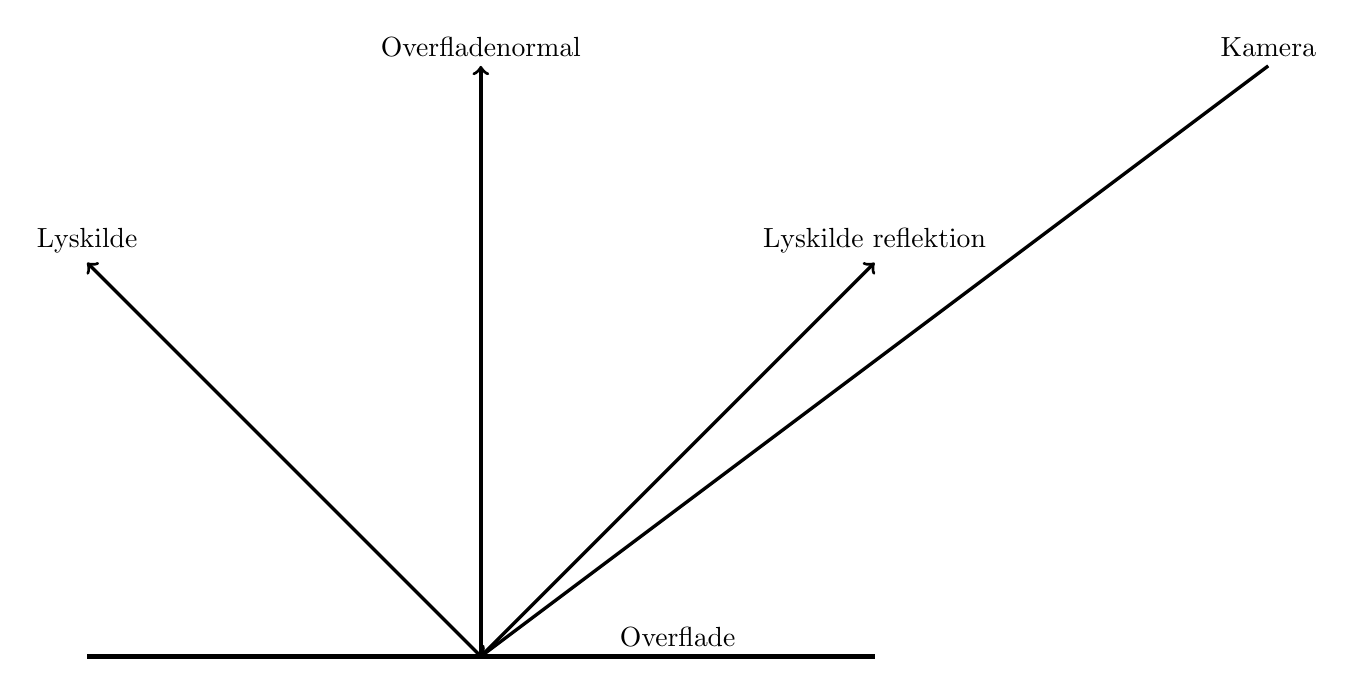
\begin{tikzpicture} [scale=2.5]
    \draw [ultra thick] (1,2) -- (5, 2);
    \node [above] at (4,2) {Overflade};
    \draw [very thick][->] (7,5) -- (3, 2);
    \node [above] at (7,5) {Kamera};
    \draw [very thick][->] (3, 2) -- (1,4);
    \node [above] at (1,4) {Lyskilde};
    \draw [very thick][->] (3, 2) -- (3,5);
    \node [above] at (3,5) {Overfladenormal};
    \draw [very thick][->] (3, 2) -- (5,4);
    \node [above] at (5,4) {Lyskilde reflektion};
  \end{tikzpicture}
  \caption{Illustration af vektorer i phong-modellen}
\end{figure}